\documentclass[]{article}
\usepackage{graphicx}
\usepackage{xcolor}

\parindent=0pt
\usepackage[margin=0.5in]{geometry}
\usepackage{url}
\usepackage{hyperref}
\usepackage{graphicx}

\begin{document}
\pagestyle{empty}
{\large\textbf{Research Notes}}
\begin{itemize}
    \item[*] Created on Mon 04 Jan 2016 11:23:25 AM EST
    \item[*] Modified on \today
    \item[*] Author info: Boyou Zhou\\
             8 St Mary's St, PHO 340, Boston, MA 02215\\
             Email: bobzhou@bu.edu, Phone: 617-678-8480\\
\end{itemize}

\rule[-0.1cm]{7.5in}{0.01cm}\\
\noindent \textbf{Mon 04 Jan 2016 11:14:43 AM EST}
\textit{Beginner's tutorial of AXI slave logic design}

This documents gives a brief instruction of how to design an AXI slave logic on Zedboard.
 Zedboard provides two ARM cores and programmable logic.
 From here, ps stands for GPP, ARM in this case, pl for programmable logic.\ 

Ps and Pl are connected with AXI ports. In this design, our logic talks to the
ps with AXI ports.\ ps looks at the logic as memory blocks. More strictly, the
ps visit the logic registers as memory units. On the ps side, I used a full
linux, Linaro Linux as the os for ps. The programs are run on the ps interfacing
the memory units through AXI ports, $/dev/mem$

Here are the tutorials to the design.
\indent		\begin{itemize}
			\item \textit{Start Linux}
			\url{http://fpga.org/2013/05/24/yet-another-guide-to-running-linaro-ubuntu-desktop-on-xilinx-zynq-on-the-zedboard/}
			\item \textit{AXI Slave Logic}
			\url{http://www.fpgadeveloper.com/2014/08/creating-a-custom-ip-block-in-vivado.html}
			\item \textit{Visit Memory Block}
			\url{http://fpga.org/2013/05/28/how-to-design-and-access-a-memory-mapped-device-part-one/}
        \end{itemize}

The device tree design, we do not include adv7511.dtsi in zynq-zed-adv7511.dtsi

\noindent \textbf{Thu 07 Jan 2016 12:38:46 PM EST}
\textit{Papers related to security}
\begin{itemize}
	\item side channel detection \cite{longo2015soc} 
	\item encoding methods \cite{chakraborti2015trivia} 
	\item radio security breach \cite{genkin2015stealing}
	\item PUF \cite{aysu2015end} \cite{maes2015secure} \cite{herder2014physical} \cite{devadas2010secure}
	\item SAT \cite{saha2015improved}
	\item TRNG \cite{haddad2015physical}\cite{suh2007physical}\cite{herder2014trapdoor}
	\item new tech \cite{suh2003efficient}
	
\rule[-0.1cm]{7.5in}{0.01cm}\\
\\
	\item coprocessor \cite{roy2015lightweight} 
	\item break RSA on Intel chip \cite{bhattacharya2015watches}
	\item accelerating homomorphic encryption \cite{doroz2015accelerating}
	\item memory verification and encryption, verification ensures the
adversary changes in the machine states. Encryption protects the off-chip
memory\cite{suh2003efficient}

\end{itemize}

some explanation
\begin{itemize}
	\item \cite{herder2014trapdoor}TRNG: safely extract the keys from biometric source
\end{itemize}

\rule[-0.1cm]{7.5in}{0.01cm}\\
\noindent \textbf{Mon 01 Feb 2016 09:55:39 AM EST}
\textit{Architecture people working on security}

\begin{itemize}
	\item Srini Devdas (MIT) \url{https://scholar.google.com/citations?user=-yrzguMAAAAJ&hl=en}
	\item Edward Suh (Cornell) \url{https://scholar.google.com/citations?user=neO3vFYAAAAJ&hl=en&oi=ao}~\cite{chen2015execution}
	\item Mohit Tiwari (U T Austin)
	\item Simha Sethumadhavan (Columbia)
	\item Tim Sherwood (UCSB)
	\item Dawn Song (U C Berkeley)
\end{itemize}

In the homomorphic computation, somewhat homomorphic function evaluation needs to be reviewed.\textbf{SHF}
\begin{itemize}
	\item \cite{chen2015execution} gives the 
\end{itemize}

\rule[-0.1cm]{7.5in}{0.01cm}\\
\noindent \textbf{Mon 22 Feb 2016 01:59:29 PM EST}
\textit{papers on architecture security}
\begin{itemize}
	\item \cite{wang2014timing} RSA attacks: each RSA decoding will result in
memory access. Thus the number of access in memory is the hamming distance of
RSA keys.
	\item \cite{ismail2015improving} 
	\item \cite{ancajas2014fort} thread model: HTs attacks one of the cores and
propagate information to other cores.  
        \begin{itemize}
            \item data scrambling
            \item dynamic packet certificate
            \item node obfuscation
        \end{itemize}
    \item \cite{liu2015ghostrider} 
        \begin{itemize}
            \item split the memory into three types, normal memory, encrypted memory and oblivious memory
            \item use software-directed scratchpad instead of implicit cache access
            \item deterministic processor pipeline against timing attacks
        \end{itemize}
\end{itemize}

\rule[-0.1cm]{7.5in}{0.01cm}\\
\noindent \textbf{Mon 22 Feb 2016 01:59:29 PM EST}
\textit{papers on architecture security}
\begin{itemize}
    \item \cite{diguet2007noc} Threat models:
        \begin{itemize}
            \item a write access in the secure area to modify the system behavior
            \item covert attacks
                \begin{itemize}
                    \item extraction of information
                        \begin{itemize}
                            \item RSA fault injection\cite{pellegrini2010fault} 
                            \item AES attack\cite{moradi2006generalized}
                            \item DPA \cite{kocher2011introduction}
                        \end{itemize}
                    \item communication between different applications \cite{wang2012efficient}
                \end{itemize}
            \item denial of service:
                \begin{itemize}
                    \item replay: wastes of bandwidth
                    \item incorrect path: introduce erroneous paths
                    \item deadlock: the use of packets with paths that intentionally create deadlocks
                    \item livelock: introduce packets that can never reach the end so that they stay turning in the network
                \end{itemize}
        \end{itemize}
\end{itemize}

\rule[-0.1cm]{7.5in}{0.01cm}\\
\noindent \textbf{Tue 08 Mar 2016 02:28:51 PM EST}
\begin{itemize}
    \item SNI - \textit{Secure Network Interface} 
        \begin{itemize} 
            \item DoS
            \item Unauthorized Read Access(Information Extraction) and unauthorized write access (Hijacking){\color{red}more literature review}
        \end{itemize}        
    \item bus-based control~\cite{diguet2007noc}
        \begin{itemize}
            \item overflow checking
            \item path based identification
            \item local access checking
            \item statistics
        \end{itemize}
    \item secure memory access \cite{goossens2008hardwired} extending \cite{fiorin2007data}
        \begin{itemize}
            \item design of Data Protection Units (DPUs) managed by Network Security Manager(NSM)
            \item memory security \cite{gebotys2003security}
            \item anti-side channel \cite{evain2005noc}
        \end{itemize} 
\end{itemize}

Memory Related Stuff
\begin{itemize}
    \item \cite{fiorin2007data} designed a module in memory call Data
Protection Unit. It protects requested accesses to the memory blocks through a
lookup of the access rights.
    \item \cite{gebotys2003security} prevents attacks which can obtain data
from communication network. Since keys are often updated from time to time. Noc
needs to secure the key exchanges on the network.
\end{itemize}

\begin{itemize}
	\item \cite{kocher2011introduction} introduction to differential power analysis
	\item \cite{pellegrini2010fault} RSA attack, retrieve the private key with fault based  
\end{itemize}


\rule[-0.1cm]{7.5in}{0.01cm}\\
\noindent \textbf{CSET}
\begin{itemize}
	\item metric security evaluation
	\begin{itemize}
		\item \textit{A Metric for the Evaluation and Comparison of Keylogger
		Performance}The paper provide a framework to assess the performance of
		mobile device keylogger.  The metric can measure the effectiveness of
		the software keyboard typing.
		\item \textit{DACSA:A Decoupled Architecture for Cloud Seucrity
		Analysis} The paper proposes an out-of-VM cloud analysis architecture.
		The framework measure the VM execution from the supervisor side for
		evaluating the security. The evaluation is the Ops/Sec on CPU and memory
		for different VMs.
		\item \textit{Effective Entropy:Security-Centric Metric for Memory
		Randomization Techniques} Effective entropy is a metric of indicating
		adversary workload and comparison between different kinds of
		randomization.
	\end{itemize}
	\item testing related papers 
	\begin{itemize}
		\item \textit{Safe and Automated Live Malware Experimentation on Public
		Testbenches} The paper is about testing methods for detections of
		malware during communication. They propose containment policies for
		testing malware by copy the observations and data gathered in malware
		analysis and put them locally for studying. It also includes emulation
		of testing environments.
		\item \textit{TESTREX: a Testbed for Repeatable Exploits} This paper
		designed a new testbed for packing and running applications with their
		environments, injecting exploits and monitoring their success. TESTREX
		combines the applications and their environments together for testing.
	\end{itemize}
\end{itemize}

\rule[-0.1cm]{7.5in}{0.01cm}\\
\noindent \textbf{WESS}
\begin{itemize}	
	\item \textit{A Novel Attack on a FPGA based True Random Number Generator}
	HT designed in the TRNG of FPGA to make the random number incident
	triggering rate rise from 0.5 to 0.75.
	\item \textit{CHEF:A Configurable Hardware Trojan Evaluation Framework}
\end{itemize}

\begin{figure}
	\centering
	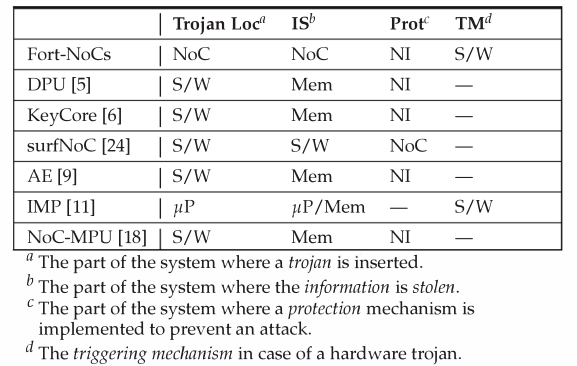
\includegraphics[width=4in]{img/defense-comparison.png}
	\caption{defense comparison}
\end{figure}

From~\cite{ancajas2014fort,js2015runtime}
\begin{itemize} 
	\item DPU		~\cite{fiorin2008secure}
	\item KeyCore	~\cite{gebotys2003framework}
	\item surfNoC	~\cite{wassel2013surfnoc}
	\item AE		~\cite{kapoor2013security}
	\item IMP		~\cite{king2008designing}
	\item NoC-MPU	~\cite{porquet2011noc}
\end{itemize}
\bibliography{week1}{}
\bibliographystyle{plain}
\end{document}

